%% Commands for TeXCount
%TC:macro \cite [option:text,text]
%TC:macro \citep [option:text,text]
%TC:macro \citet [option:text,text]
%TC:envir table 0 1
%TC:envir table* 0 1
%TC:envir tabular [ignore] word
%TC:envir displaymath 0 word
%TC:envir math 0 word
%TC:envir comment 0 0
% chktex-file 1
% chktex-file 8

%manuscript, acmsmall, acmlarge, acmtog, sigconf, siggraph, sigplan, sigchi, sigchi-a
\documentclass[sigchi-a,screen,nonacm,language=german]{acmart}

%% Date
\usepackage{datetime}
\day=23 \month=12 \year=2022  
\newdateformat{monthYear}{\monthname[\THEMONTH] \THEYEAR}

%% Quotes
\usepackage[]{csquotes}

%% Figures
\usepackage{subcaption}

%% Acronyms
\usepackage[nohyperlinks,nolist]{acronym}

%% Theorems
\theoremstyle{acmdefinition}

\newtheorem{requ}{Research Question}
\def\requautorefname{RQ}

\newtheorem{rein}{Research Interest}
\def\reinautorefname{RI}

\renewcommand*{\figureautorefname}{Fig.}

%% TikZ
\usepackage{pgfplots}
\pgfplotsset{width=7cm,compat=1.8} 
\usetikzlibrary{intersections,calc}
\pgfkeys{/pgf/number format/1000 sep={}}

%Einrückung unterbunden
%\setlength{\parindent}{0pt}



%%
%% \BibTeX command to typeset BibTeX logo in the docs
\AtBeginDocument{%
  \providecommand\BibTeX{{%
    \normalfont B\kern-0.5em{\scshape i\kern-0.25em b}\kern-0.8em\TeX}}}



%% Rights management information.  This information is sent to you
%% when you complete the rights form.  These commands have SAMPLE
%% values in them; it is your responsibility as an author to replace
%% the commands and values with those provided to you when you
%% complete the rights form.
\setcopyright{none}
\acmDOI{}
\acmPrice{}
\acmISBN{}

%% These commands are for a PROCEEDINGS abstract or paper.
% \acmConference
%   [SG-MCI: HAI (Prof. Dr. Raphaela Groten)]
%   {TH Köln, Medieninformatik Ma., Spezielle Gebiete der Mensch-Computer-Interaktion: HAI (SG-MCI: HAI) bei Prof. Dr. Prof. Dr. Raphaela Groten}
%   {SoSe 2022}
%   {Gummersbach, Deutschland}


\settopmatter{printacmref=false,printfolios=true}

%%
%% Submission ID.
%% Use this when submitting an article to a sponsored event. You'll
%% receive a unique submission ID from the organizers
%% of the event, and this ID should be used as the parameter to this command.
%%\acmSubmissionID{123-A56-BU3}

%%
%% The majority of ACM publications use numbered citations and
%% references.  The command \citestyle{authoryear} switches to the
%% "author year" style.
%%
%% If you are preparing content for an event
%% sponsored by ACM SIGGRAPH, you must use the "author year" style of
%% citations and references.
\citestyle{acmauthoryear}

%%
%% end of the preamble, start of the body of the document source.
\begin{document}

%%
%% The "title" command has an optional parameter,
%% allowing the author to define a "short title" to be used in page headers.
\title{Ability-Based Design für die inklusive und zugängliche Gestaltung von sozio-technischen Systemen}
\subtitle{Posterabstract für das Projekt 1 \enquote{Barrierefreies Begleitsystem im ÖPNV für Menschen mit kognitiven Beeinträchtigungen} im Schwerpunkt \acf{hci}}
\subtitlenote{Im Rahmen des Advanced Seminar im Medieninformatik Master an der TH Köln bei Prof. Dr. Mirjam Blümm im Wintersemester 2022/23}

%%
%% The "author" command and its associated commands are used to define
%% the authors and their affiliations.
\author{Finn Nils Gedrath}
\authornote{Beide Autor:innen haben zu gleichen Teilen zu dieser Arbeit beigetragen.}
\orcid{0000-0002-8697-7669}
\email{finn_nils.gedrath@smail.th-koeln.de}
\affiliation{%
  \institution{TH Köln}
  \streetaddress{Steinmüllerallee 1}
  \city{Gummersbach}
  \country{Germany}
  \postcode{51643}
}

\author{Katrin Hartz}
\authornotemark[2]
\email{katrin.hartz@smail.th-koeln.de}
\affiliation{%
  \institution{TH Köln}
  \streetaddress{Steinmüllerallee 1}
  \city{Gummersbach}
  \country{Germany}
  \postcode{51643}
}



%%
%% By default, the full list of authors will be used in the page
%% headers. Often, this list is too long, and will overlap
%% other information printed in the page headers. This command allows
%% the author to define a more concise list
%% of authors' names for this purpose.
\renewcommand{\shortauthors}{Finn Nils Gedrath und Katrin Hartz}

%%
%% The abstract is a short summary of the work to be presented in the
%% article.
%\begin{abstract}
%\end{abstract}

%%
%% The code below is generated by the tool at http://dl.acm.org/ccs.cfm.
%% Please copy and paste the code instead of the example below.
%%
\begin{CCSXML}
<ccs2012>
   <concept>
       <concept_id>10003120.10011738.10011773</concept_id>
       <concept_desc>Human-centered computing~Empirical studies in accessibility</concept_desc>
       <concept_significance>500</concept_significance>
       </concept>
   <concept>
       <concept_id>10003120.10003121.10003129</concept_id>
       <concept_desc>Human-centered computing~Interactive systems and tools</concept_desc>
       <concept_significance>500</concept_significance>
       </concept>
   <concept>
       <concept_id>10003120.10011738.10011772</concept_id>
       <concept_desc>Human-centered computing~Accessibility theory, concepts and paradigms</concept_desc>
       <concept_significance>300</concept_significance>
       </concept>
   <concept>
       <concept_id>10003120.10003121.10003122</concept_id>
       <concept_desc>Human-centered computing~HCI design and evaluation methods</concept_desc>
       <concept_significance>300</concept_significance>
       </concept>
 </ccs2012>
\end{CCSXML}


\ccsdesc[500]{Human-centered computing~Empirical studies in accessibility}
\ccsdesc[500]{Human-centered computing~Interactive systems and tools}
\ccsdesc[300]{Human-centered computing~Accessibility theory, concepts and paradigms}
\ccsdesc[300]{Human-centered computing~HCI design and evaluation methods}

%%
%% Keywords. The author(s) should pick words that accurately describe
%% the work being presented. Separate the keywords with commas.
%\keywords{tbd}


%%
%% This command processes the author and affiliation and title
%% information and builds the first part of the formatted document.
\maketitle

%%
%% Acronyms
\begin{acronym}
  % see https://www.namsu.de/Extra/pakete/Acronym.html
  \acro{iso}[ISO]{International Organization for Standardization}
  \acro{iese}[Frauenhofer IESE]{Fraunhofer-Institut für Experimentelles Software Engineering}
  \acro{gi}[GI]{Gesellschaft für Informatik}
  \acro{acm}[ACM]{Association for Computing Machinery}
  \acro{ieee}[IEEE]{Institute of Electrical and Electronics Engineers}
  \acro{hci}[HCI]{Human-Computer Interaction}
  \acro{abd}[ABD]{Abillity-based Design}
  \acro{ud}[UD]{Universal Design}
  \acro{ui4a}[UI4A]{User Interfaces for All}
  \acro{bmg}[BMG]{Bundesministerium für Gesundheit}
\end{acronym}

%%
%% Citations

% non-breaking space      -> ~
% half-non-breaking space -> \,
% n-dash                  -> --

% S. (Seite)            -> p. (page)          -> [][p.~15]
% S. (Seiten)           -> pp. (pages)        -> [][pp.~15--16]
% Z. (Zeile)            -> l. (line)          -> [][l.~48]
% Z. (Zeilen)           -> ll. (lines)        -> [][ll.~48--63]
% f. (Folgend)          -> f. (following)     -> [][p.~15\,f.]
% ff. (Fort-Folgende)   -> ff. (following)    -> [][p.~15\,ff.]
% siehe                 -> see                -> [see][]
% vgl. (vergleiche)     -> cf. (confer)       ->
% u.a. (unter anderem)  -> i.a. (inter alia)  -> [see i.\,a.][]
% u.a. (und andere)     -> et al. (et aliae)  ->

\section{Einleitung}
\label{sec:einleitung}

Barrieren treten in Form von Usability Problemen in der Interaktion mit sozio-technischen Systemen auf.
Jede:r Nutzer:in hat seine eigenen Fähigkeiten, Erfahrungen, Erfordernisse, die sich auch situativ und temporär verändern können. % <= Source: Microsoft?
Bei der Gestaltung eines interaktiven Systems müssen diese Fähigkeiten berücksichtigt werden. Besonders wenn ein System für Menschen mit nicht normativen bio-psychischen Fähigkeiten gestaltet werden muss, kann eine darauf nicht angepasste Umwelt zu fehlender Partizipation, also einer Barriere führen. % <= Eventuell ICF bio-psycho-soziales Model der Behinderung (Fußnote?)

Im Gestaltungsprozess müssen diese Anforderungen an das System ermittelt werden. Eine Methode, ein hohes Maß an Zugänglichkeit zu erreichen, ist das \ac{abd}. Innerhalb dieses Posterabstracts wird das \ac{abd} grundlegend in den Forschungsbereich der zugänglichen menschen-zentrierten Gestaltung eingeordnet. Es werden dann exemplarisch zwei Feldanwendungen %Feldstudien?? 
vorgestellt, bei denen nach den Prinzipien des \ac{abd} gearbeitet wurde. Es werden die Erfahrungen der Forschenden vorgestellt und die Unterschiede der beiden Projekte diskutiert. Diese Ergebnisse sollen in einem Poster aufgearbeitet werden.

% Forschungsfrage!!!!
%Ziel ist es ein wissenschaftliches Poster zu gestalten, welches die Prinzipien des \ac{abd} anhand zweier Feldstudien genauer erläutert. Dazu wird deren Vorgehensweise analysiert und miteinander vergleichen. Anhand dessen soll eine eigene Vorgehensweise aufgestellt werden, die wir in unserem Projekt verfolgen werden. 


\section{Abillity-Based Design als Design-for-One Ansatz}
\label{sec:abd}



% Es gibt mehrer Methoden a11y zu gestaltne

% - design-for-all => UD (-> Produktdesign + Bau)
% - design-for-one => ABD (UI4A streichen)

Grundsätzlich lassen sich Designphilosophien für die inklusive Gestaltung sozio-technischer Systeme in \emph{design-for-all} und \emph{design-for-one} Ansätze unterteilen. Bei dem \ac{ud}-Ansatz (design-for-all; Anwendung vor allem im Produktdesign und Bau von physischen Umwelten) wird versucht, ein statisches System zu entwickeln, welches für die größt-mögliche Menge an Nutzer:innen ohne spezielle Adaptoren nutzbar ist. Im Gegensatz dazu kann eine deutlich größere Menge potentieller Nutzer:innen erreicht werden, wenn sich das System an die Erfordernisse, Präferenzen, demografischen Daten und Voreinstellungen anpasst \citep{benyon-etal:inclusive-design:2001}.

\citet{stephandis:ui-all:2001} bezeichnete den \ac{ui4a} Ansatz als Paradigmenwechsel in der \ac{hci}. Es sollte nicht mehr eine Benutzungsschnittstelle entwickelt werden, sondern mehrere parallel oder so, dass sie sich nach bestimmten Richtwerten selbstständig anpasst. Ziel ist es, den in \autoref{fig:adaptors:adaptor-system} benötigten Adapter durch ein sich anpassbares System zu ersetzen (siehe \autoref{fig:adaptors:ability-system}).

\begin{marginfigure}
    \centering

    \begin{subfigure}[b]{\marginparwidth}

        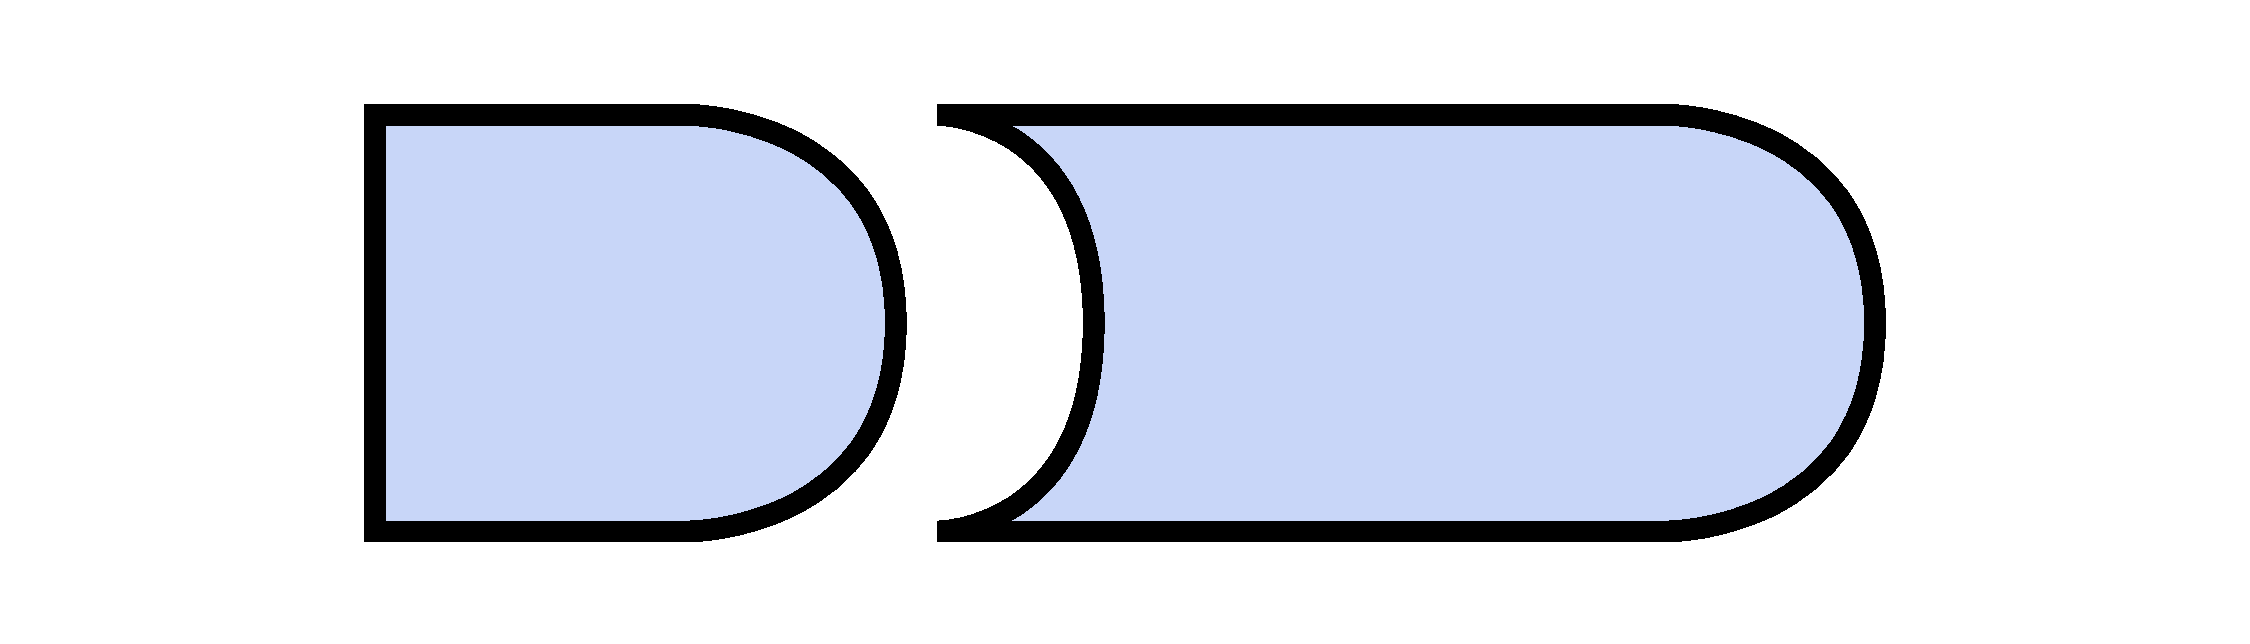
\includegraphics[width=\linewidth]{media/figures/ability-based_user-system.pdf}
        \caption{User / System}\label{fig:adaptors:user-system}
        
    \end{subfigure}
    \hfill
    \begin{subfigure}[b]{\marginparwidth}

        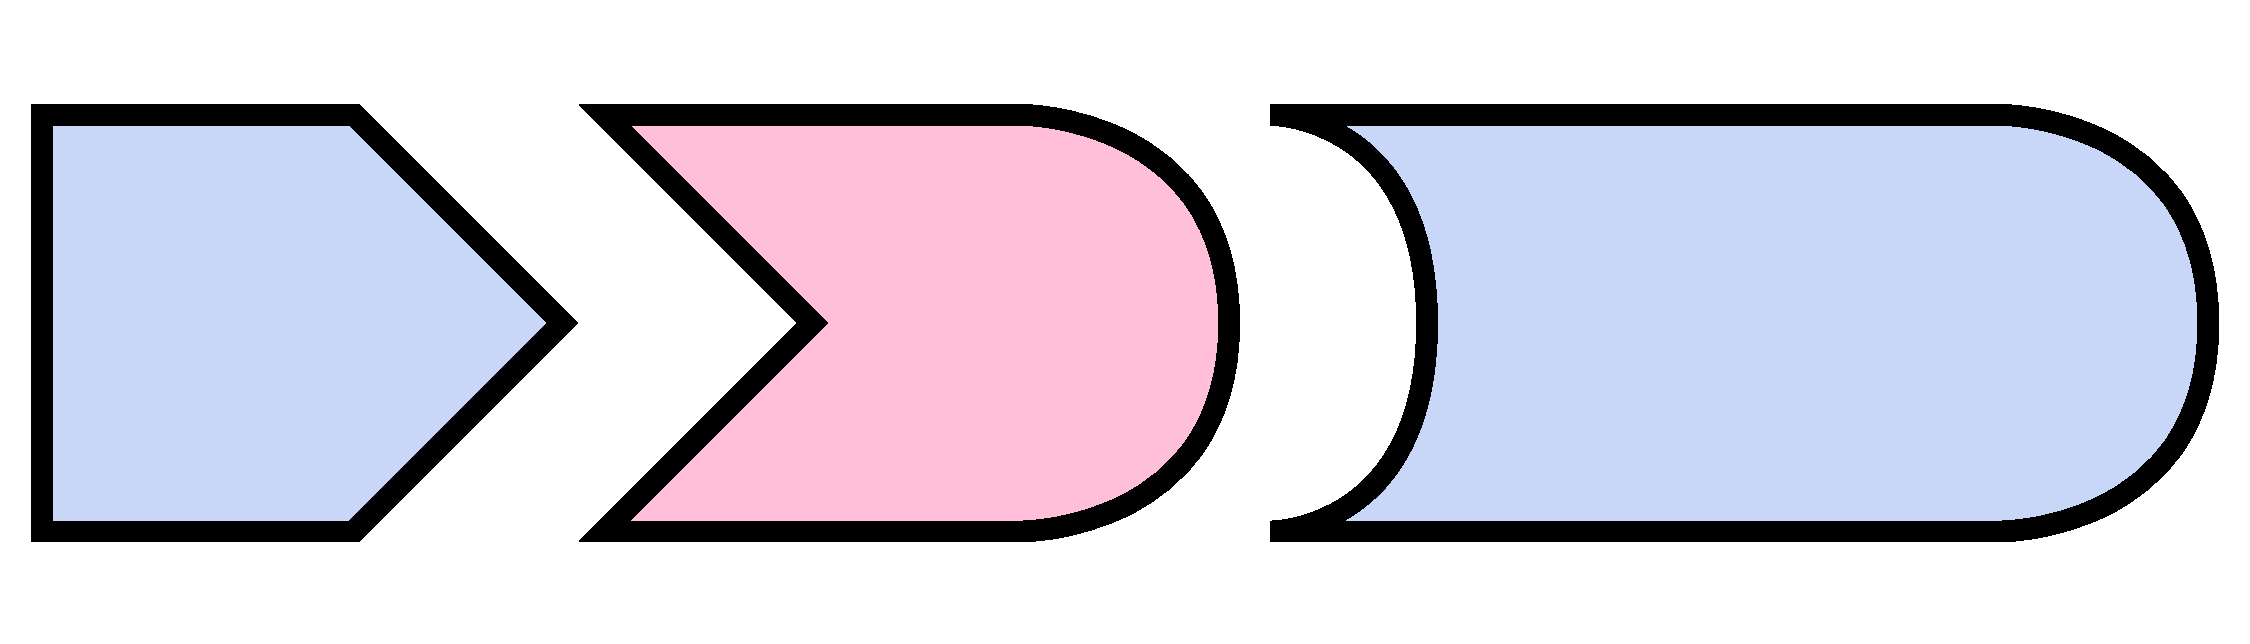
\includegraphics[width=\linewidth]{media/figures/ability-based_user-adaptor-system.pdf}
        \caption{User / Adaptor / System}\label{fig:adaptors:adaptor-system}
        
    \end{subfigure}
    \hfill
    \begin{subfigure}[b]{\marginparwidth}

        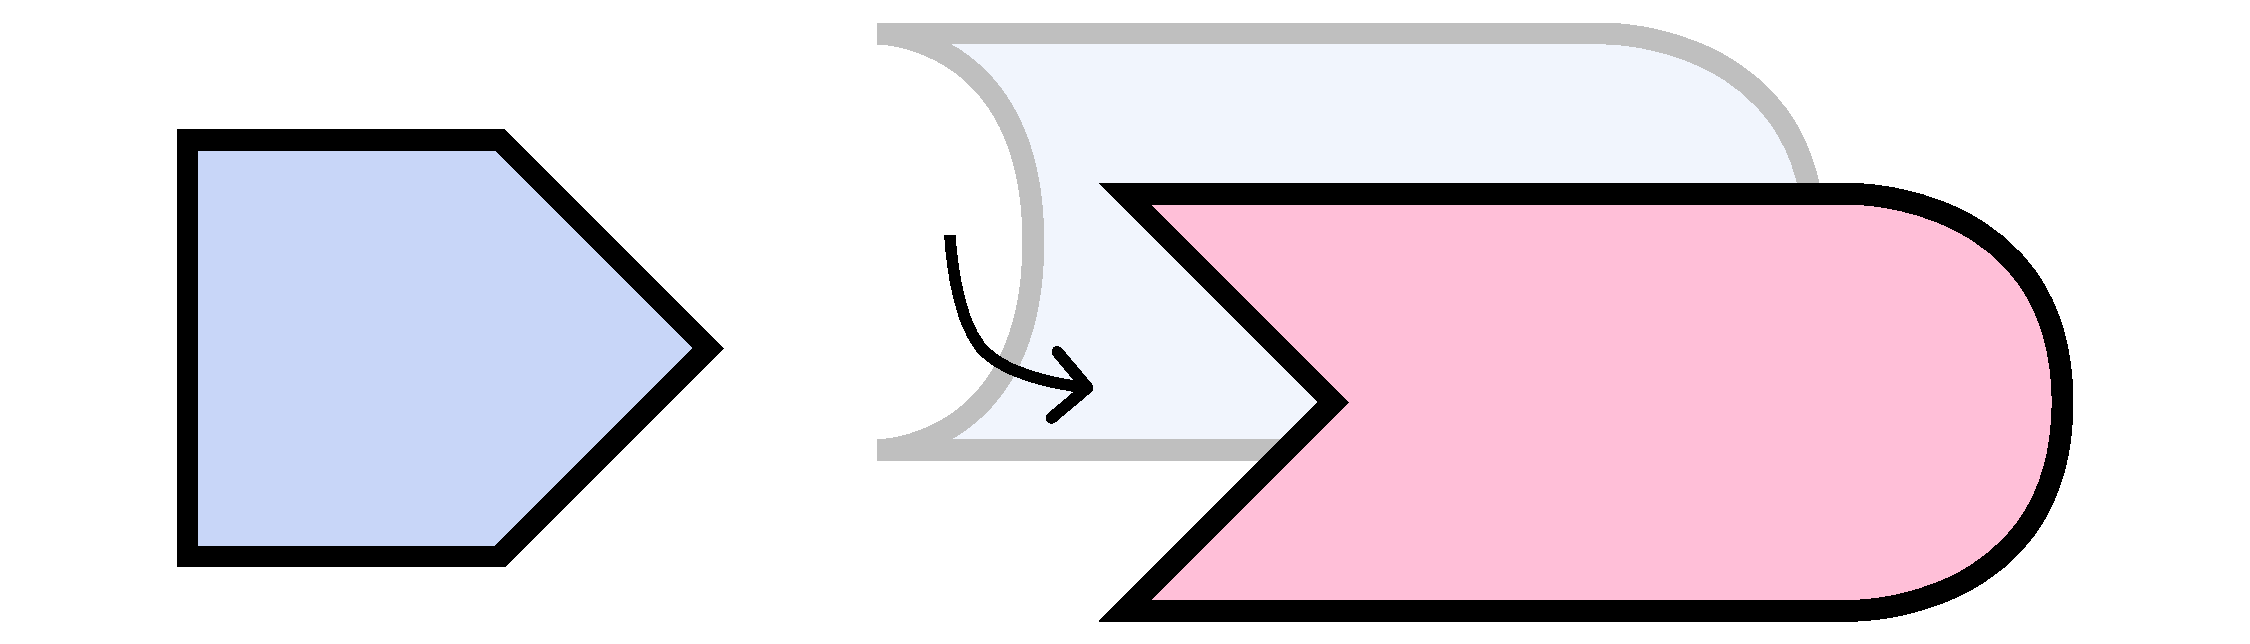
\includegraphics[width=\linewidth]{media/figures/ability-based_user-ability-system.pdf}
        \caption{User / Ability-based System}\label{fig:adaptors:ability-system}
        
    \end{subfigure}

    \caption{Der Unterschied zwischen einem System, bei dem (a) der:die Benutzer:in die vom System geforderten Fähigkeit hat oder (b) einen eigenen Adaptor braucht, und (c) einem System, das sich den Fähigkeiten des:der Benutzer:in anpasst \citep[Eigene Darstellung nach][S.~4]{wobbrock-etal:ability-based-design:2011}.}
    \label{fig:adaptors}
\end{marginfigure}

Als eine Erweiterung des \ac{ui4a}-Ansatzes kann das \emph{\acf{abd}} angesehen werden. Auch hier soll sich die Benutzungsschnittstelle nach bestimmten Eigenschaften anpassen. Das \ac{abd} verschiebt die Betrachtungsweise. Es wird nicht mehr die Beeinträchtigung eines:r jeweiligen Benutzers:in fokussiert, sondern seine:ihre immer noch zur Verfügung stehenden perzeptorischen, kognitiven und motorischen Fähigkeiten. \citet{wobbrock-etal:ability-based-design:2011} stellt mehrer Prinzipien vor, die bei der Arbeit nach dem \ac{abd} berücksichtigt werden sollten   \citep[vgl.][]{wobbrock-etal-ability-based-design:2018,wobbrock-etal:ability-based-design:2011}:

\begin{itemize}
    \item \textbf{Ability} \\
        Designers will focus on ability not \emph{dis}-ability, striving to leverage all that users \emph{can} do.
    \item \textbf{Accountability} \\
        Designers will respond to poor performance by changing systems, not users, leaving users as they are.
    \item \textbf{Adaptation} \\
        Interfaces may be self-adaptive or user-adaptable to provide the best possible match to users’ abilities.
    \item \textbf{Transparency} \\
        Interfaces may give users awareness of adaptations and the means to inspect, override, discard, revert, store, retrieve, preview, and test those adaptations.
    \item \textbf{Performance} \\
        Systems may regard users’ performance, and may monitor, measure, model, or predict that performance.
    \item \textbf{Context} \\
        Systems may proactively sense context and anticipate its effects on users’ abilities.
    \item \textbf{Commodity} \\
        Systems may comprise low-cost, inexpensive, readily available commodity hardware and software.
\end{itemize}


\section{Praktische Anwendungen des ABD}
\label{sec:vorstellung}

\defcitealias{alsaleem:2020:adaptive-outdoor-activities}{Paper~I}
\defcitealias{Schneider:2022:Aid-watch}{Paper~II}

Als Ergebnis der Literatur-Recherche wurden zwei Paper ausgewählt, die im Folgenden vorgestellt
werden:

\begin{itemize}
    \item \citetalias{alsaleem:2020:adaptive-outdoor-activities}: Ahmad Alsaleem, Ross Imburgia, Andrew Merryweather, Jeffrey Rosenbluth, Stephen Trapp, and Jason Wiese. 2020. Applying Ability-Based Design Principles to Adaptive Outdoor Activities. \emph{In Proceedings of the 2020 ACM Designing Interactive Systems Conference} (Eindhoven, Netherlands) (\emph{DIS~’20}). Association for Computing Machinery, New York, NY, USA, 1–12.
    
    \item \citetalias{Schneider:2022:Aid-watch}: Rahel Mirijam Schneider, Hauke Steffen Wendt, and Alexander Kuon. 2022. AID-Watch - Smartwatch for People with Cognitive Impairments. In \emph{Proceedings of Mensch Und Computer 2022} (Darmstadt, Germany) (\emph{MuC~’22}). Association for Computing Machinery, New York, NY, USA, 622–624.
\end{itemize}


\subsection{Paper I: Adaptive Outdoor Activities}
\label{sec:vorstellung:lit-1}



%%% Kontext

\citet{alsaleem:2020:adaptive-outdoor-activities} entwickelten im Nutzungskontext von Sportaktivitäten im Freien ein System für Menschen mit motorischen Beeinträchtigungen. Im Besonderen soll es Menschen mit Tetraplegie\footnote{Menschen mit \emph{Teraplegie} (ICD G82.5) können bspw. durch Verletzungen des Rückenmarks im Wirbelkanal die Muskeln in Armen, Beinen und Rumpf nicht bewegen \citep{bmg:icd-code}} ermöglichen, Extremsportarten durchführen zu können. Die Autor:innen stellen für diese Menschengruppe eine besondere Relevanz solche Systeme zu entwickeln hervor, da neben den physischen Barrieren auch soziale Barrieren im Besonderen zu beobachten seien.

%%% Ziel

Konkret wurde der Fokus auf zwei verschiedene Sportarten gelegt: Zum einen dem Skifahren und dem Segeln (siehe \autoref{fig:alsaleem2020}). Die Autor:innen erkennen das Problem in bestehenden (auch kommerziell erhältlichen) Systemen, dass das selbstständige Handeln mit den unterstützenden Geräten nur eingeschränkt möglich ist. Ziel ist es, die Autonomie der Nutzer:innen zu stärken \citep[vgl.][S.~2]{alsaleem:2020:adaptive-outdoor-activities}.



%%% Blick auf ABD
%"This approach shifts the burden of accessibility away from the user to technology designers and developers." (p.1)

Der Projektverlauf ist sehr eng an den Prinzipien des \ac{abd} orientiert. In einem Zeitraum von fünf Jahren beginnend 2015 wurde in mehreren Iterationen und Test-Einsätzen die beiden Systeme entwickelt.

%%% Restriktionen
%Spezifische Einschränkung der Körperfunktion (-> ausschließlich ) + Spezifischer Anwendungsfall
%5 Jahre Entwicklung / seit 2015 (p.1)




%%% Methodik (ABD)
%Challenging: Mapping of ABD principles (p.1)
%=> Outdoor Environment (context of use) was hard to define/predict => risk assessment (p.1)
%=> Gestaltungslösung: collaboration btw control partner + main user (p.1) -> Shared control (p. 4)

%-> "medical and social factors" gleichermaßen betrachten

%Designansatz: Shared-Control
%-> Person mit motorischer Beeinträchtigungen
%-> erfahrender Sportlehrer

\citet{alsaleem:2020:adaptive-outdoor-activities} orientierten sich im Projektverlauf sehr stark an den Prinzipien des \ac{abd}. Sie haben feststellen müssen, dass die Einhaltung der \ac{abd}-Prinzipien sowohl für Tetra-Ski als auch Tetra-Sail nur über den Design-Ansatz \emph{Shared-Control} möglich ist (siehe \autoref{fig:alsaleem2020}). Hierbei führt der:die Nutzer:in zusammen mit einem:einer Sportlehrer:in die Aktivität aus. Dadurch wird ermöglicht, dass der:die erfahrende Sportlehrer:in die Entscheidungen und Aktionen des:der Nutzer:in verfeinern bis verändern kann (siehe \emph{Adaptation}). So können auch Umgebungsvariablen wie Wetterverhältnissen (siehe \emph{Context}) oder die Veränderung von Fähigkeiten durch einen Lerneffekt mit einbezogen werden \citep[vgl.][S.~4-5]{alsaleem:2020:adaptive-outdoor-activities}.

Die alleinige Nutzung der Aktivität ist für die Nutzenden zu gefährlich. Zwar konnte aus den Erfahrungen anderer Projekte mit ihren ermittelten Barrieren und Anforderungen zurückgegriffen werden, jedoch sind sie für diesen Nutzungskontext nicht ausführlich genug oder können pro Nutzer:in variieren.


\begin{marginfigure}
    \centering

    \begin{subfigure}[b]{\marginparwidth}

        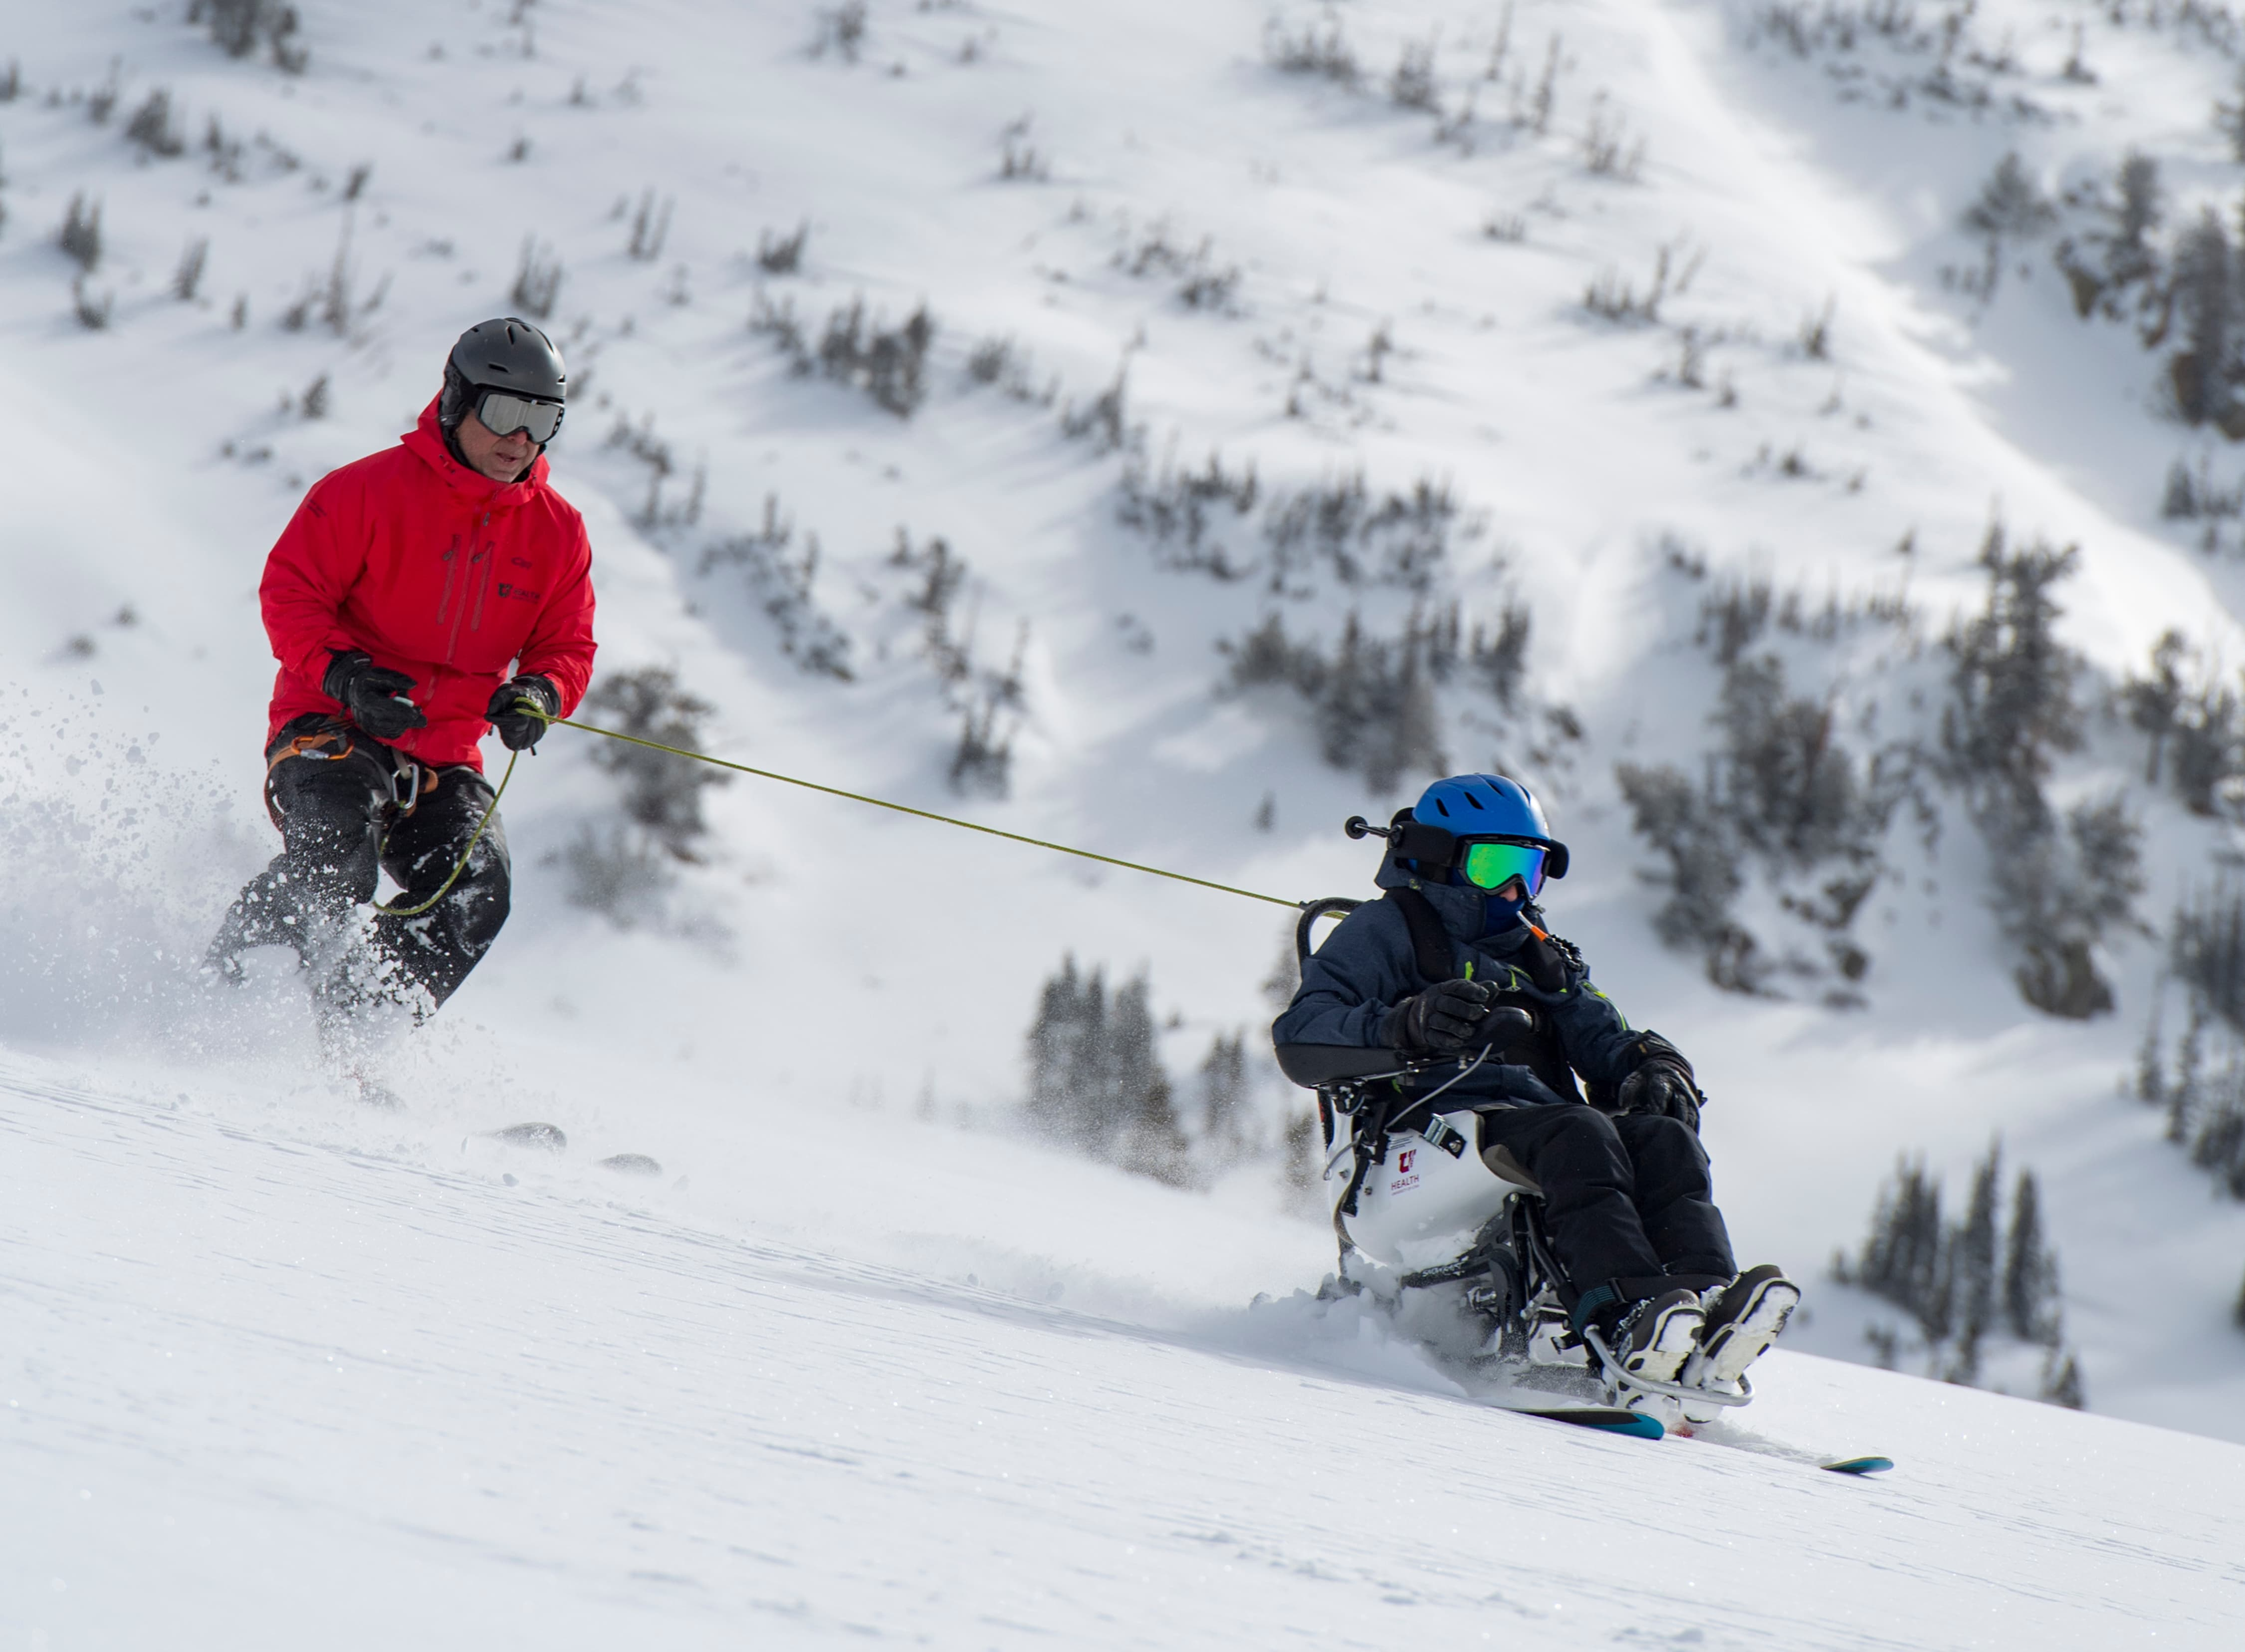
\includegraphics[width=\linewidth]{media/alsaleem2020_tetra-ski.jpg}
        \caption{Tetra-Ski}\label{fig:alsaleem2020:tetra-ski}
        
    \end{subfigure}
    \hfill
    \begin{subfigure}[b]{\marginparwidth}

        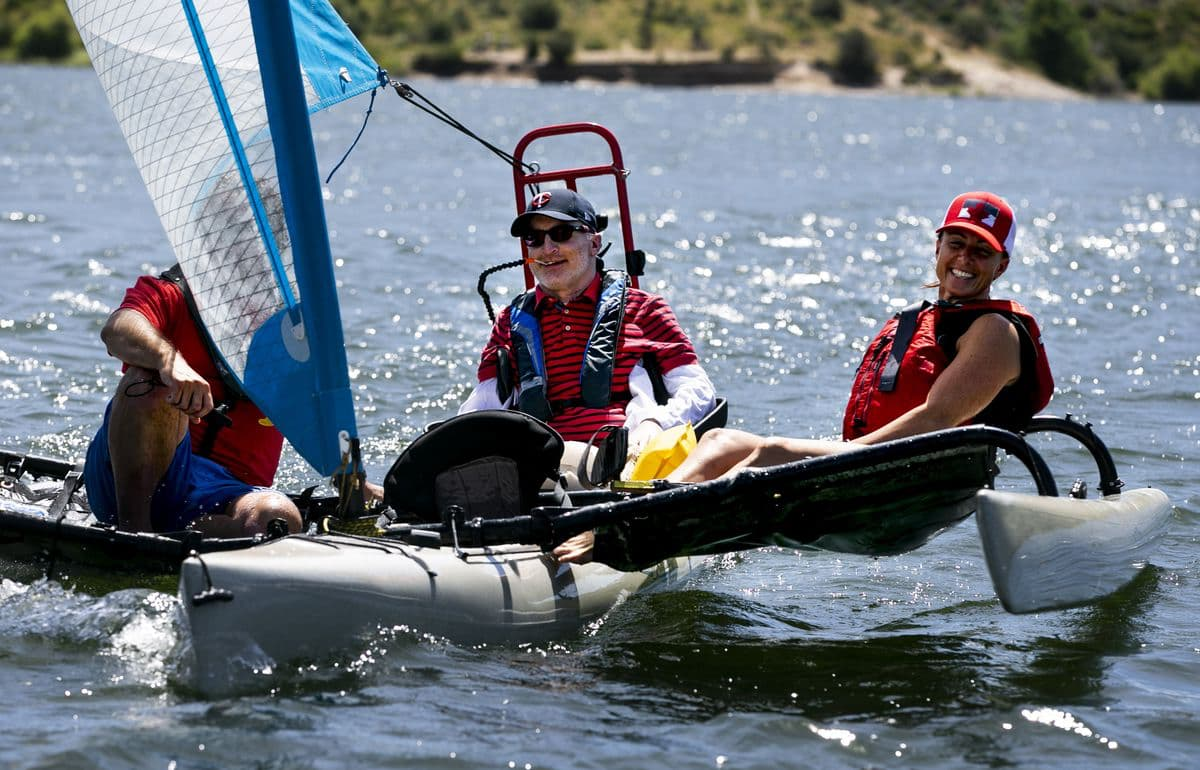
\includegraphics[width=\linewidth]{media/alsaleem2020_tetra-sail.jpg}
        \caption{Tetra-Sail}\label{fig:alsaleem2020:tetra-sail}
        
    \end{subfigure}

    \caption{Projekt-Ergebnisse von \citet{alsaleem:2020:adaptive-outdoor-activities}. In beiden Projekten wurde der Shared-Control Ansatz umgesetzt (Bildrechte bei den jeweiligen Autoren, wie durch \citeauthor{alsaleem:2020:adaptive-outdoor-activities} genannt).}
    \label{fig:alsaleem2020}
\end{marginfigure}

% independence / performance

Das Prinzip der \emph{Adaption} war für die \citet{alsaleem:2020:adaptive-outdoor-activities} nur schwer umzusetzen, da hier der Tetra-Ski/-Sail auf die eigenen Fähigkeiten der Nutzer:innen angepasst werden müsste. Zum einen entstand hier ein zeitlicher Aufwand, das jeweilige Gerät zu verändern und zum anderen passt nicht jede Steuerung physisch zu dem Gerät. Um die Gebrauchstauglichkeit während schneller Handlungen zu gewährleisten, wurde ein vereinfachtes gegenüber eines hoch-individualisierbaren Interface präferiert. Die Autor:innen mussten hier Prinzipien des \ac{abd} bewusst widersprechen, um die Sicherheit und Umsetzbarkeit der Nutzung zu gewährleisten.


%%% Learnings

Die Autor:innen erkennen als Learning aus dem Projekt, dass Shared-Control in Nutzungskontexten, die nur schwer beschrieben werden können, als eine sinnvolle Methode an. Sie sehen Ähnlichkeiten zum Wizard-of-Oz Prototyping, um in einer günstigen und für alle Beteiligten sicheren Umgebung die sich durch situative Barrieren verändernden Anforderungen zu ermitteln. Die Rolle des:der Begleitenden kann in Anschlussprojekten durch das System selbst erfolgen. Nutzende haben \citet{alsaleem:2020:adaptive-outdoor-activities} auf der anderen Seite gespiegelt, dass sie das Shared-Control Konzept und die daraus resultierenden Eingriffe als beruhigend wahrgenommen haben.

Das iterative Vorgehen in der Projektarbeit hat es zudem ermöglicht, die sich untereinander ausschließenden und beeinflussenden Prinzipien zu vereinen. Die \ac{abd}-Prinzipien wurden für jede Iteration neu priorisiert, um auf neue Erkenntnisse reagieren zu können und den Entscheidung der Gestaltungsvarianten zu erleichtern \citet[vgl.][S.~8]{alsaleem:2020:adaptive-outdoor-activities}.

%Die Autor:innen empfehlen die Prinzipien des \ac{abd} umd ie Prinzipien Autonomie, Kompetenz und Shared-Control zu erweitern.

\subsection{Paper II: AID-Watch}
\label{sec:vorstellung:lit-2}

% - Kontext
Menschen mit kognitiven Einschränkungen fällt es häufig schwer, komplexe Informationen aufzunehmen, zu verstehen und zu verarbeiten. % Beleg ??
In ihrem Projekt legen die Autor:innen den Fokus auf Menschen, die aufgrund ihrer kognitiven Einschränkungen nicht in der Lage sind, die Uhr zu lesen und daher bei der Planung ihres Tagesablaufs auf zusätzliche Unterstützung angewiesen sind. Feste Zeitpläne, die mit individuellen Fotos, Icons oder Bildern visualisiert werden, helfen diesen Menschen dabei ein besseres Verständnis für Zeit und Abläufe zu entwickeln \citep{Schneider:2022:Aid-watch}.

% - Ziel
Durch eine Digitalisierung dieser analogen Ablaufpläne und der Wiedergabe auf einer Smartwatch sollen die Nutzer:innen die Reihenfolge verschiedener Events besser verfolgen können. AID-Watch bietet durch die interaktive Anzeige eine einfache Zugänglichkeit des Tagesablaufs und die Möglichkeit, die Fähigkeit der Nutzer:innen, selbständig Termine und Events wahrzunehmen, zu verbessern. Dies ermöglicht es ihnen, ihren Tag unabhängiger zu gestalten.

% - Restriktionen
Da das Testen des Systems sehr zeitaufwendig ist, beschränkten sich die Autor:innen zunächst nur auf eine Testperson mit Lese-Rechtschreibstörung\footnote{Menschen mit einer \emph{Lese-Rechtschreibstörung} (ICD F81.0) haben eine Beeinträchtigung in Lese- und/oder Rechtschreibfertigkeiten, die nicht allein durch das Entwicklungsalter, Visusprobleme oder unangemessene Beschulung erklärbar sind \citep{bmg:icd-code}}.
Im späteren Projektverlauf sollen noch weitere Tests mit verschiedenen Testpersonen mit unterschiedlichen kognitiven Fähigkeiten durchgeführt werden.

% - Methodik (ABD)
\citet{Schneider:2022:Aid-watch} berücksichtigen bei ihrem Vorgehen die Prinzipien der \ac{abd}, gehen jedoch nicht explizit darauf ein.
Das System wird an die Fähigkeiten der Zielgruppe wie beispielsweise das Verständnis visueller Darstellungen angepasst (siehe \emph{Ability}). Dies wurde im weiteren Projektverlauf mehrfach getestet und optimiert. 

\begin{marginfigure}
    \centering

    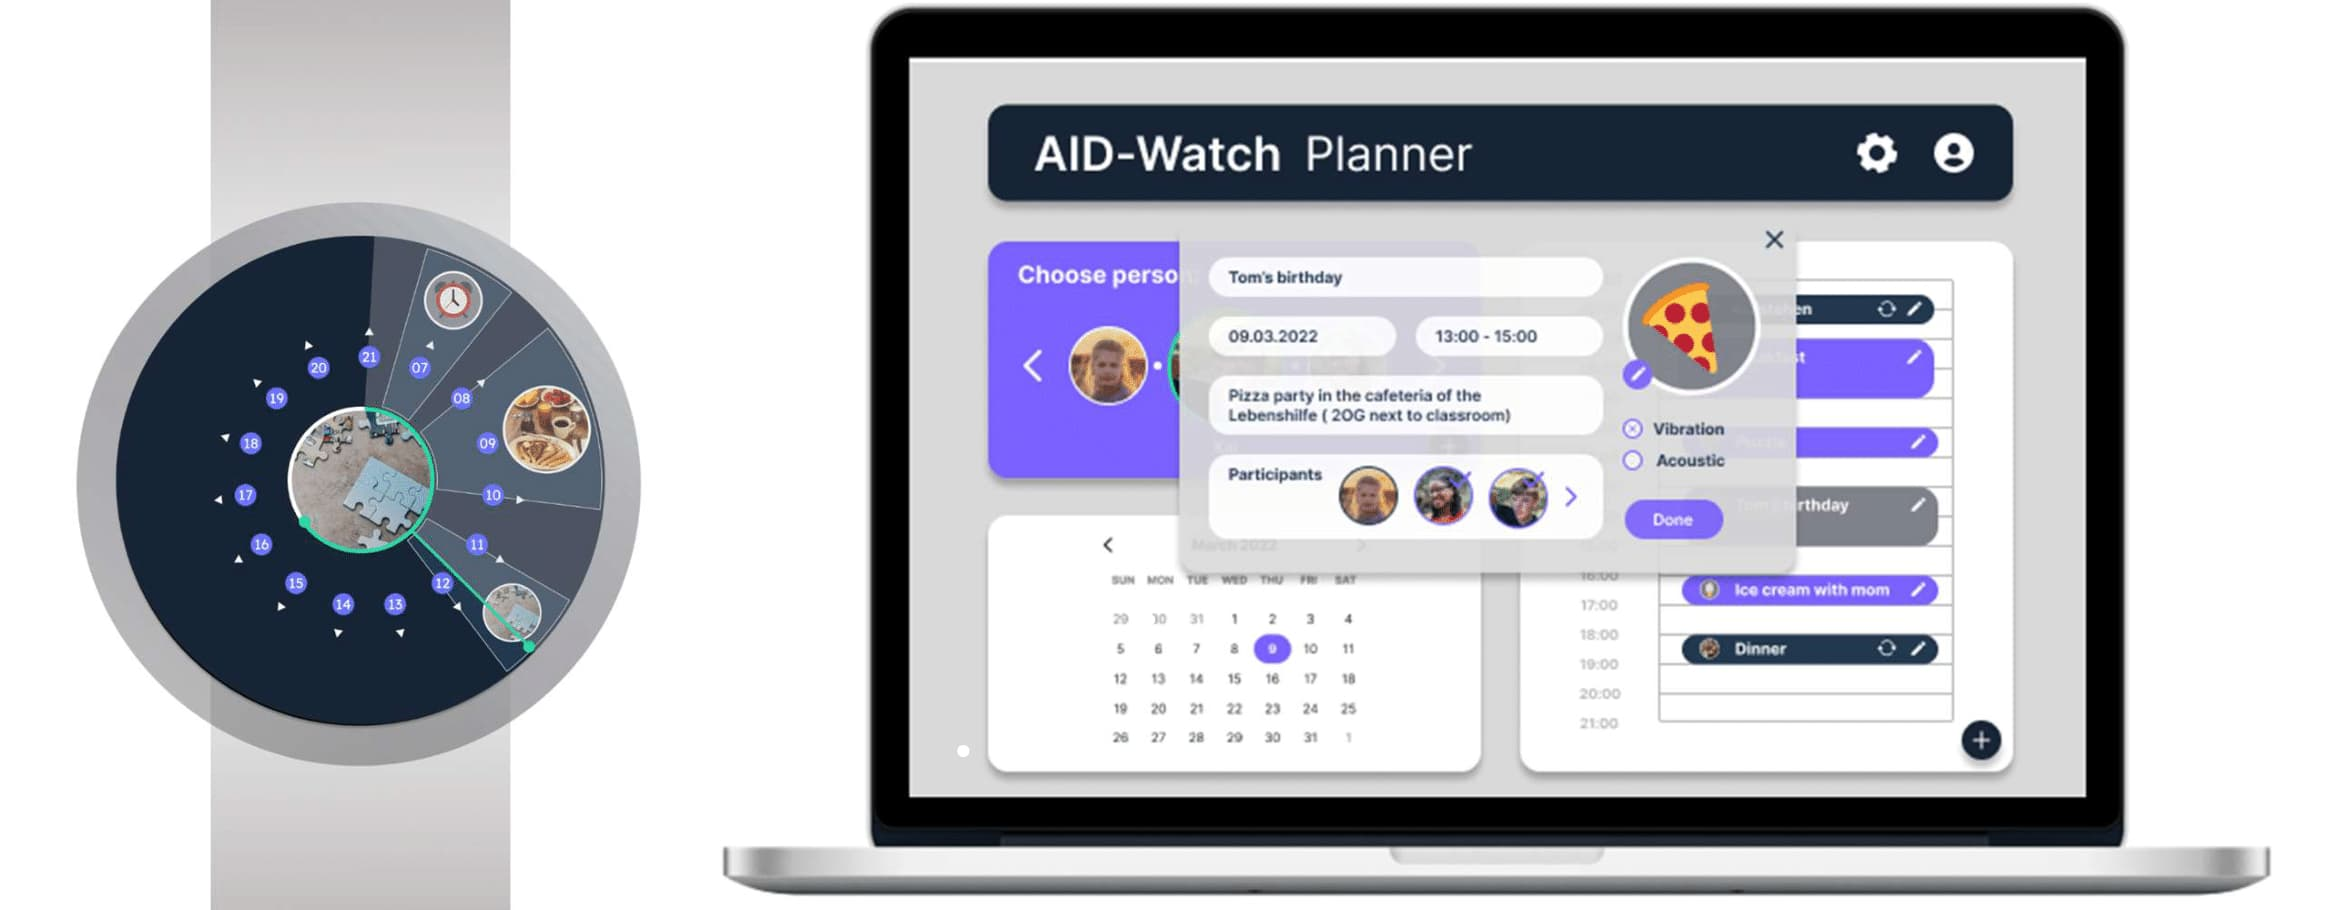
\includegraphics[width=\linewidth]{media/kuon2022_AID-Watch.jpg}

    \caption{Projekt-Ergebnisse von \citet{Schneider:2022:Aid-watch}: Die AID-Watch für den:die Nutzer:in mit kognitiven Beeinträchtigungen mit dem dazugehörigen Planner für Betreuer:innen.}
    \label{fig:schneider2022}
\end{marginfigure}

% - Learnings: Keep / Drop / Try
Aus diesem Grund wurde auch von einem 12h Ziffernblatt auf eine Displayansicht gewechselt, die den Tag in 16h und 8h unterteilt (siehe \emph{Accountability}). Das hat den Vorteil, dass der Tages- und Schlafrhythmus verdeutlicht wird und alle Events in der korrekten Reihenfolge und dem dazugehörigen Symbol angezeigt werden können. %Durch das iterative Vorgehen wurde das verbreitete 12h Ziffernblatt verworfen, da bei dieser Anzeige das Dispaly mitten am Tag aktualisiert und verändert werden muss. Dies hat bei der Testperson zu Verständnisproblemen geführt. Stattdessen wird der Tag in 16h und 8h unterteilt (siehe \emph{Accountability}).
%Events werden je nach Dauer Das 16h-Display zeigt alle Events des Tages mit den dazugehörigen Symbolen an. Der Eventbereich und das Symbol werden größer, je mehr Zeit ein Event in Anspruch nimmt. 
Durch akustische und haptische Signale wird der:die Nutzer:in auf den Beginn eines Events aufmerksam gemacht. %Innerhalb der ersten drei Minuten wird das Symbol ganzflächig auf dem Display angezeigt, danach ist es mit einer Progress-anzeige in der Mitte zu sehen %% umforlulieren.... 
Um den Tagesablauf zu verdeutlichen, läuft ein Zeiger mit und zeigt auf das aktuelle Event, bereits abgeschlossene Events werden ausgegraut.

Obwohl der Fokus der AID-Watch Anzeige auf den Events und deren Reihenfolge liegt, wird zusätzlich die Uhrzeit mit Ziffern angezeigt. So können Nutzer:innen regelmäßige Events mit den Uhrzeiten verknüpfen und diese lernen. 

Der erste User-Test hat gezeigt, dass Symbole teilweise unterschiedlich von den Nutzer:innen interpretiert werden. Aus diesem Grund sollen betreuende Personen die Möglichkeit bekommen, die Events in Absprache mit den Nutzer:innen mit Symbolen oder persönlichen Bildern zu visualisieren (siehe \emph{Adaption}). Dies ist in der AID-Watch Planner Anwendung möglich, dort sollen alle Events angelegt, verwaltet und geplant werden (siehe \autoref{fig:schneider2022}). 


% - User Testing(?) -> Wie wurde es angenommen?
Laut \citet[][]{Schneider:2022:Aid-watch} war die Testperson durch AID-Watch in der Lage, Termine selbstständig einzuhalten. Ebenso hat sich die Wahrnehmung von Ablauf und Dauer der einzelnen Events verbessert.
Diese neue Unabhängigkeit der Testperson mindert den Stress der betreuenden Personen, was wiederum die Pflege und Individualisierung des digitalen Tagesablaufs rechtfertigt. 
  

\section{Zusammenfassung}
\label{sec:zusammenfassung}

Aus den vorgestellten Papern können Schlüsse für die eigene Anwendung des \ac{abd} gezogen werden. Zum einen wurde in \citetalias{alsaleem:2020:adaptive-outdoor-activities} die Anpassung der Priorisierung der \ac{abd}-Prinzipien für jede Gestaltungsiteration nach einer abgeschlossenen Evaluation für sinnvoll erachtet. Sowohl \citetalias{alsaleem:2020:adaptive-outdoor-activities} als auch \citetalias{Schneider:2022:Aid-watch} haben die Liste der \ac{abd}-Prinzipien um andere erweitert. Diese müssen dann mit in der Priorisierung berücksichtigt werden.

\citetalias{Schneider:2022:Aid-watch} hat im bisherigen Projekt-Status nur eine:n Untersuchungsteilnehmende:n in der Entwicklung berücksichtigt. Um eine Adaption des Systems für mehrere Nutzende zu gewährleisten, muss eine heterogene Gruppe an Menschen und deren Erfordernisse betrachtet werden. \citetalias{alsaleem:2020:adaptive-outdoor-activities} nutzt als Methode das Wizard-of-Oz Prototyping, um die Anforderungen an die Anpassbarkeit des Systems zu testen. Hierbei wird durch eine begleitende Person das System in Absprache an die sich verändernden situativen Gegebenheiten und Fähigkeiten angepasst.

% Key Takeaways:
% - Priorisierung der ABD-Prinzipien pro Iteration sinnvoll
% - gibt es Punkte/Prinzipien, die für das Projekt wichtiger sind und somit über den ABD-Prinziopien stehen?
% - Es muss mit mehreren unterschiedlichen Untersuchungsteilnehmenden getestet werden
% - Methoden wie Wizard-of-Oz sind sinnvoll um situative Anforderungen zu ermitteln


%\section{Fazit und Ausblick}
%\label{sec:fazit-ausblick}
%Auf unserem Poster möchten wir darstellen welche \ac{abd} Prinzipen berücksichtigt wurden, wie in den Feldstudien vorgegangen wurde und in wie fern diese Vorgehensweise auf unser Projekt bzw. allgemein auf Projekte anzuwenden ist. 
% aus Forschungssicht
% aus P1 sicht



%%
%% The acknowledgments section is defined using the "acks" environment
%% (and NOT an unnumbered section). This ensures the proper
%% identification of the section in the article metadata, and the
%% consistent spelling of the heading.
%\begin{acks}
%  tbd.
%\end{acks}

%%
%% If your work has an appendix, this is the place to put it.
%\appendix


%%
%% The next two lines define the bibliography style to be used, and
%% the bibliography file.
\bibliographystyle{ACM-Reference-Format}
\bibliography{literatur}


\end{document}
\endinput
